\section{Data Collection and Basic Analysis}
\label{sec:meth}

This section introduces \vt\ and 
discusses how we collect data from \vt\ and preprocess them.
We also present the analysis results of their basic properties, 
before delving into more advanced analysis in later sections.


\begin{table}[h!]
\centering
\footnotesize
{
\begin{tabular}{l|l}
\hline
Metadata Field & Explanation \\
\hline                            
%\cline{1-1}
{\bf name}      & submitted file name \\
{\bf link}      & where to download the file \\
{\bf timestamp} & timestamp when the submission was made \\
{\bf source\_country} & the country where the submission was made \\
{\bf source\_id} & user ID who made the submission\\
{\bf size} & file size \\
{\bf type} & file type \\
{\bf tags} & labels with more specific information for each {\bf type}\\
{\bf first\_seen} & when the same file was first submitted \\
{\bf last\_seen} & when the same file was last submitted \\
{\bf hashes} & sha1, sha256, md5, and vhash\\
{\bf ssdeep} & ssdeep digest string \\
{\bf total} & number of engines analyzing the file \\
{\bf positives} & number of engines that flagged the file as malicious \\
{\bf positives\_delta} & changes in {\bf positives} across different submissions\\
{\bf report} & detailed detection report from each AV engine \\
\hline
\end{tabular}
}
\caption{VirusTotal Metadata. 
%\footnotesize{
(Fields for each submission retrieved from VirusTotal through distribution API and their related explanation.
One file could be submitted multiple times by different users.)
%}
}
\label{tab:fields}
\end{table}


\subsection{VirusTotal}
\vt\ is a free online malware scan service.
It was founded in 2004 and was acquired by google in 2012. 
\vt\ is widely used by both normal users and anti-virus vendors.
Normal users submit suspicious files to \vt\ when they do not have any anti-virus software, 
or when they want to check for viruses possibly missed by their own anti-virus software 
or false alarms from their own anti-virus software.  
Anti-virus vendors use \vt to verify false positives and false negatives in their products.

For each submission, \vt\ applies a set of anti-virus engines to analyze it. 
\vt\ keeps information about whether the submission is labeled as malware by each engine, 
and detailed tags for identified malware from each engine. 

\vt\ provides open APIs to access and download both the metadata of all submissions and detection results.
One API, named distribution API, works like a pipe.
After a user opens the distribution API and starts to download data from \vt, 
\vt\ will keep returning metadata for latest submission to the user. 
Roughly 20 GB data can be downloaded from \vt\ through distribution API.  

\vt\ provides rich metadata.
Table~\ref{tab:fields} shows the metadata fields and their meaning.  
The original submitted files from \vt\ can be downloaded using the {\bf link} field in the metadata.

\subsection{Data Collection and Preprocessing}
We collected all metadata for all submissions to \vt\ from May 7th, 2016 to September 6th, 2016,
with a total of 151 million submissions. 
Our collected data is larger than or comparable to previous works on studying \vt~\cite{SongAPsys2016,huangvt2016bigdata}.
According to Lastline Labs~\cite{Lastline}, common lag time for an anti-virus engine to detect a new malware is two weeks.
Thus, four months' data is more than enough to analyze most malware and anti-virus engine behavior. 
In deed, we drew several meaningful conclusions with this dataset, as will be presented in the rest of the paper.

We performed our data collection using \vt{}’s distribution API.
We insert all collected metadata into a table in Cassandra~\cite{cassandra} 
using the combination of sha256, source\_id, and timestamp as the key.
We then used Spark~\cite{spark} and wrote Spark programs to efficiently analyze the vast amount of data.
All our analysis is conducted by using Spark 1.4.0 on a cluster with 19 nodes, 266 cores, and 560 GB memory. 

\begin{figure}[t!]
\begin{center}
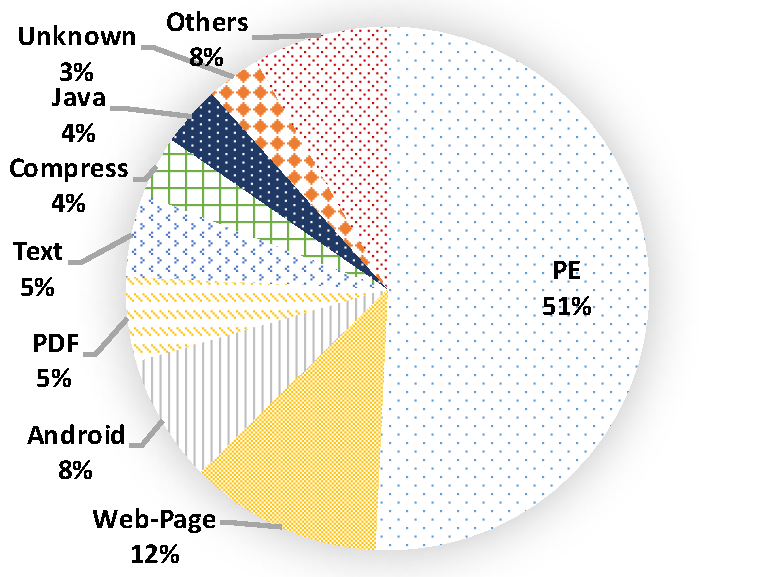
\includegraphics[width=2.in]{figure/type}
\caption{File type distributions.
%{\footnotesize{
(File types and their distributions for all VirusTotal submissions from 05/07/2016 to 09/06/2016.)
%}
}
\label{fig:type}
\end{center}
%\vspace{-0.25in}
\end{figure}


Figure~\ref{fig:type} shows the file type distribution for all submissions. 
Among all file types, Windows \textit{Portable Executable} ({\em \pe}) files, or ``Win32EXE'' and ``Win32DLL'' files, 
are the most frequently submitted type,
accounting for 51\% of all submissions.
%which conforms with a previous study~\cite{SongAPsys2016}.
Web pages and Android apps account for the second and third largest submissions, 
with 12\% and 8\% of all submissions respectively. 
Other popular file types include PDF, Text, compressed files, and Java files. 
This result shows that even though new types of malware such as Android apps have
increased significantly in recent years, 
traditional types of malwares such as \pe\ files and web pages are still the 
most commonly targeted by attackers.

Since PE files are the most common type,
we focus our study in this paper on \pe\ files 
and leave studies on other types of malwares for future. 
%If the type field for a submission is either ``Win32EXE'' or ``Win32DLL'', 
%we consider the submission is a PE file. 
In total, we collected 76 million \pe\ submissions.

\subsection{Basic Analysis}
After collecting data, we first conducted a set of analysis 
to learn various basic properties of submission files, 
submission sources, and anti-virus engines.
These properties give an overview of how real-world submissions and anti-virus enginesare like
and serve as the foundation for our more advanced analysis in the next two sections. 



\begin{figure}[t!]
\begin{center}
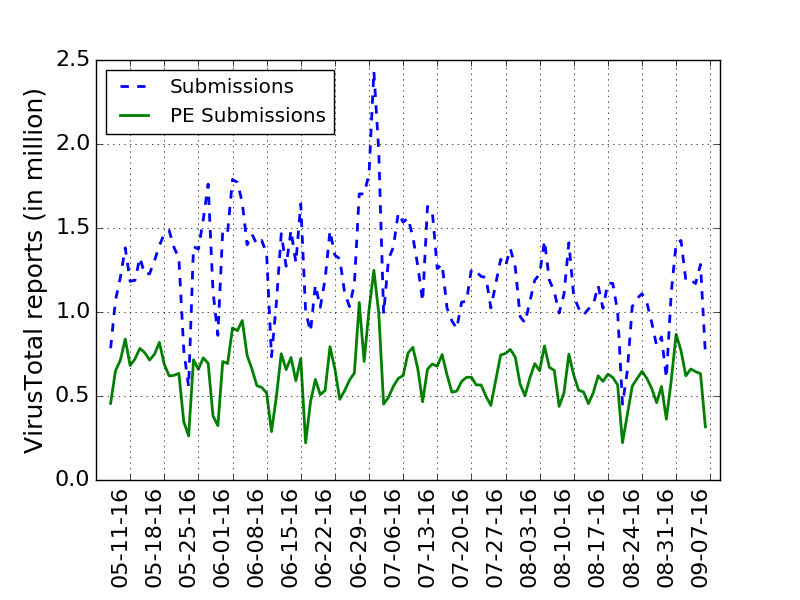
\includegraphics[width=2in]{figure/Submissions}
\caption{The number of files and PE files.
%{\footnotesize{
(The number of suspicious files and the number of PE files submitted to VirusTotal from 05/07/2016 to 09/06/2016.)
%}
}
\label{fig:subnum}
\end{center}
%\vspace{-0.25in}
\end{figure}

\begin{figure}[t!]
\begin{center}
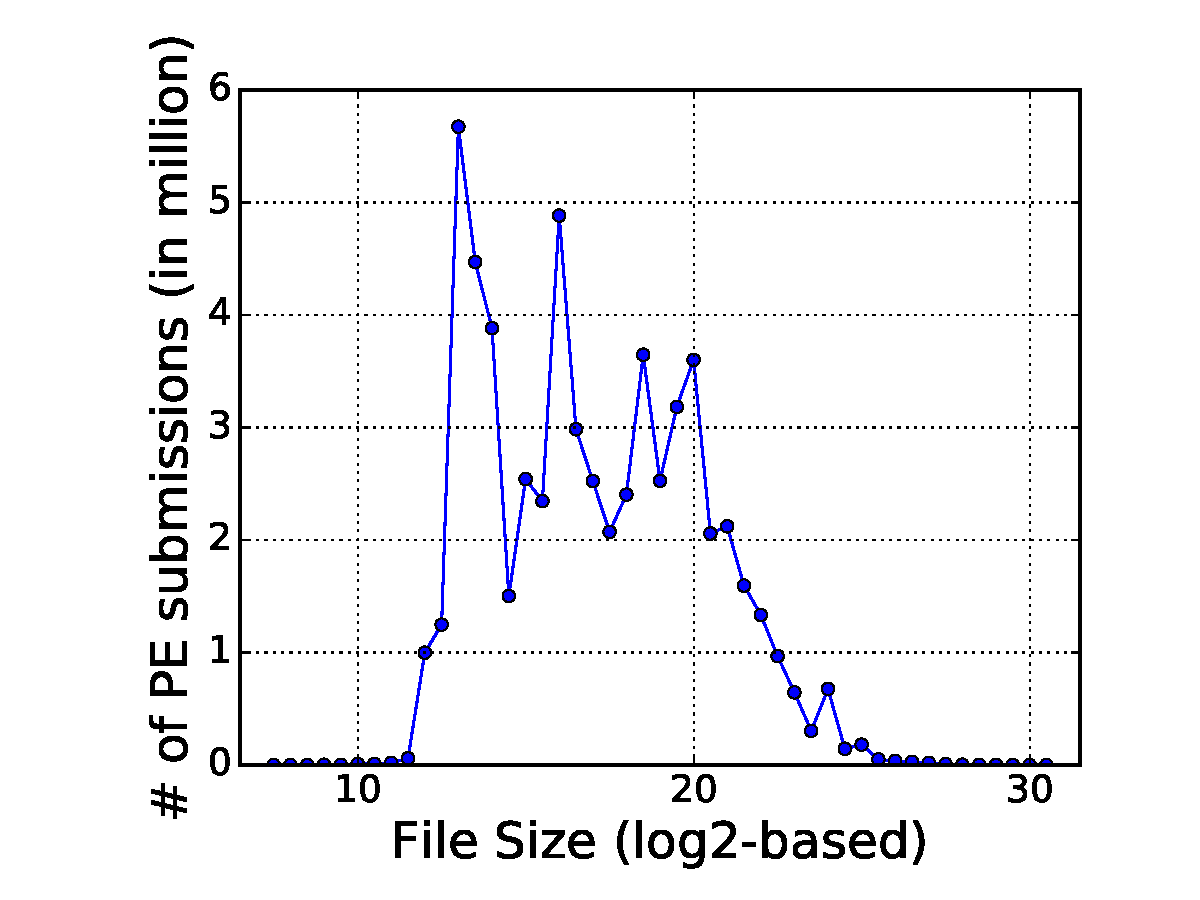
\includegraphics[width=2.5in]{figure/pesize}
\mycaption{fig:pesize}{File size distribution for PE submissions.}
{\footnotesize{(How file size distributes among all PE submissions we collect. 
Results from log2 are rounded up to nearest 0.5.)}}
\end{center}
%\vspace{-0.25in}
\end{figure}
\begin{figure}[t!]
\begin{center}
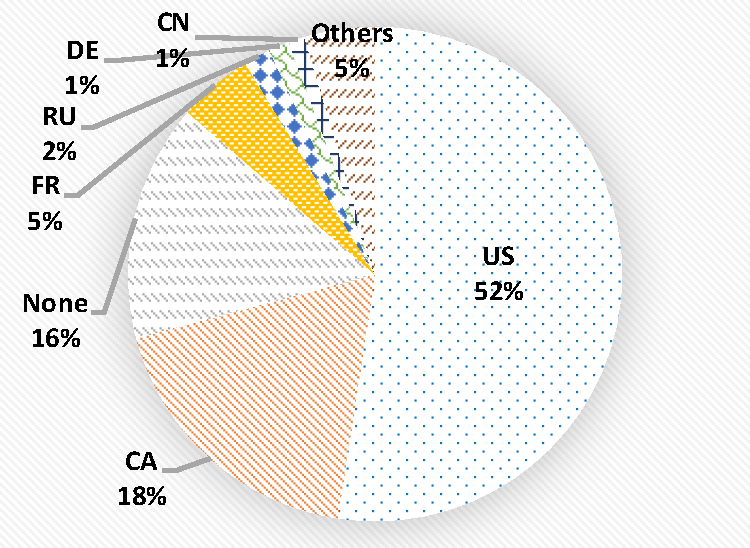
\includegraphics[width=2in]{figure/countryPie}
\caption{How PE submissions distribute among different countries.
%\footnotesize{
(Only countries with more than 1\% PE submissions are shown.)
%}
}
\label{fig:countryPie}
\end{center}
%\vspace{-0.25in}
\end{figure}

\noindent{\textit{\underline{Submission temporal, geo-location, and size distribution.}}}
Figure~\ref{fig:subnum} plots the number of submissions of all types and the number of \pe\ submissions per day 
over the whole collection period.
There are a large amount of submissions every day
and the amount of submissions is fairly stable over the whole collection period.
The same conclusion can be made to \pe\ submissions.

One PE file could be submitted more than once to VirusTotal. 
On average, each PE file was submitted 1.19 times and 6.72\% PE files were submitted more than once. 

For around 16\% of PE submission, 
\vt fails to provide their source country information. 
All other submissions are conducted from 221 countries. 
The top 6 countries in PE submission number are US, Canada, France, Russia, Germany, and China, 
as shown in Figure~\ref{fig:countryPie}.

Figure~\ref{fig:pesize} shows the file size distribution for PE submissions. 
The smallest PE file is only 187 bytes, and the largest one is more than 1\,GB. 
99.58\% of PE file fall into the range from 4\,KB to 32\,MB. 

{\bf Observation 1:} 
{\em \vt\ constantly receives large amount of submissions from all over the world. 
Most submitted files have small to middle sizes and are only submitted once, 
but some files are submitted many times.}

\begin{figure}[t!]
\begin{center}
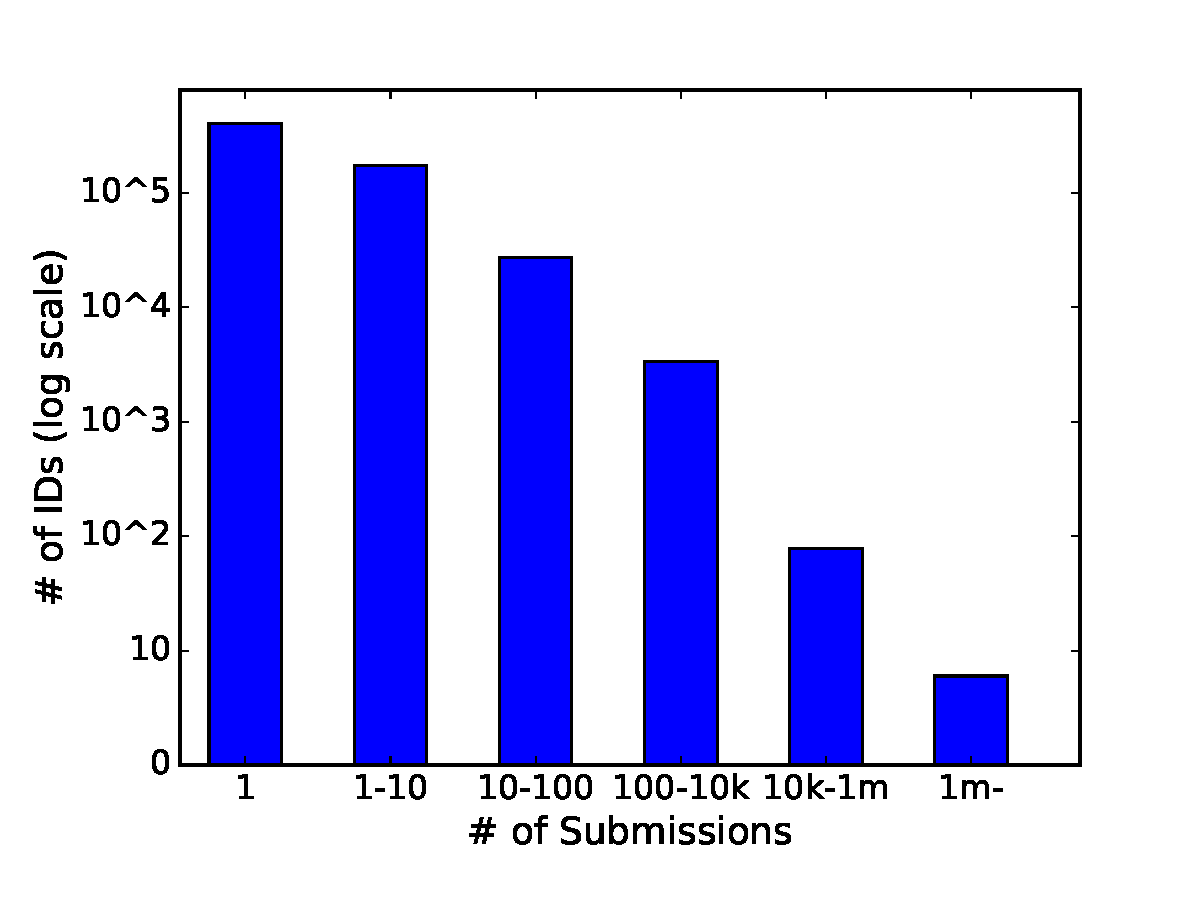
\includegraphics[width=2.5in]{figure/IDDistribution}
\mycaption{fig:iddis}{The distribution for source ids.}
{\footnotesize{(How source ids distribute among all source id groups. 
We divide groups based on PE submissions made by each source id.)}}
\end{center}
%\vspace{-0.25in}
\end{figure}
\noindent{\textit{\underline{Submission sources.}}}
Both normal users and anti-virus vendors use \vt\ to detect malwares or evaluate products.
Usually, vendors tend to make more submissions than normal users, since they need to test their products on many files.
Thus, we use the number of submissions to measure what type of users a source ID is.

We seperate the number of submissions into six categories:
one submission, one to ten submissions, ten to 100 submissions, 100 to 10000 submissions, 10000 to 1 million submissions, and larger than 1 million submissions.
Figure~\ref{fig:iddis} plots the number of source IDs in log scale in the first five categories.
\yiying{change figure X axis to 1 1-10 10-100 100-10K 10K-1Mil and change Y axis label to 0 10\^5 10\^10 etc.}
There are only 6 source IDs that have more than 1 million submissions and we suspect that these IDs are either bogus or robots 
that constantly make submissions to \vt.
For the rest, we find that the number of source IDs dramatically drops when the number of submissions is more than 100.
Thus, we categorize the source IDs as normal user if they have less than 100 submissions and as vendors if they have more than 100 submissions.

{\bf Observation 2:} 
{\em Most \vt\ users are normal users that make occasional submissions, while a small set of anti-virus vendors use \vt\ and make a huge amount of submissions.}

\begin{figure}[t!]
\begin{center}
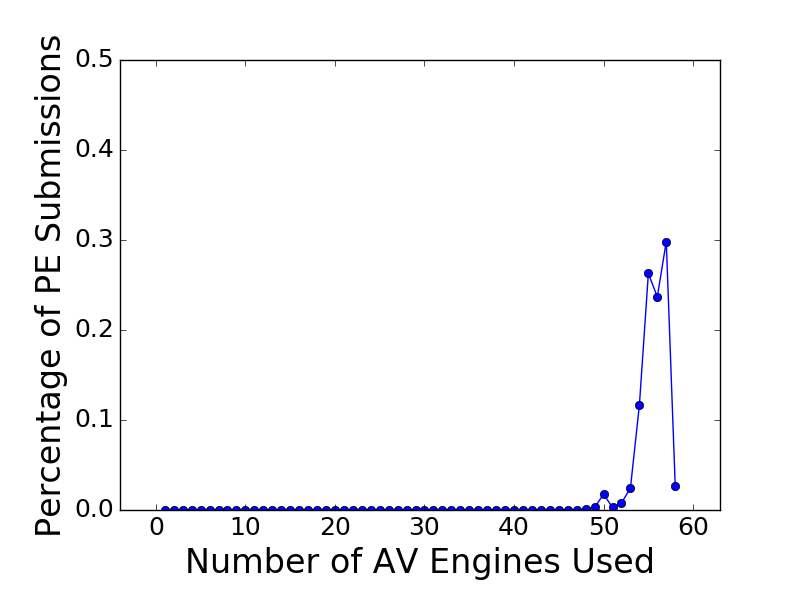
\includegraphics[width=2in]{figure/numVendor}
\caption{The distribution for the number of used anti-virus engines.
(How the number of applied anti-virus engines distributes among all PE submissions.
)
}
\label{fig:vendornum}

\end{center}
%\vspace{-0.25in}
\end{figure}
\begin{figure}[t!]
\begin{center}
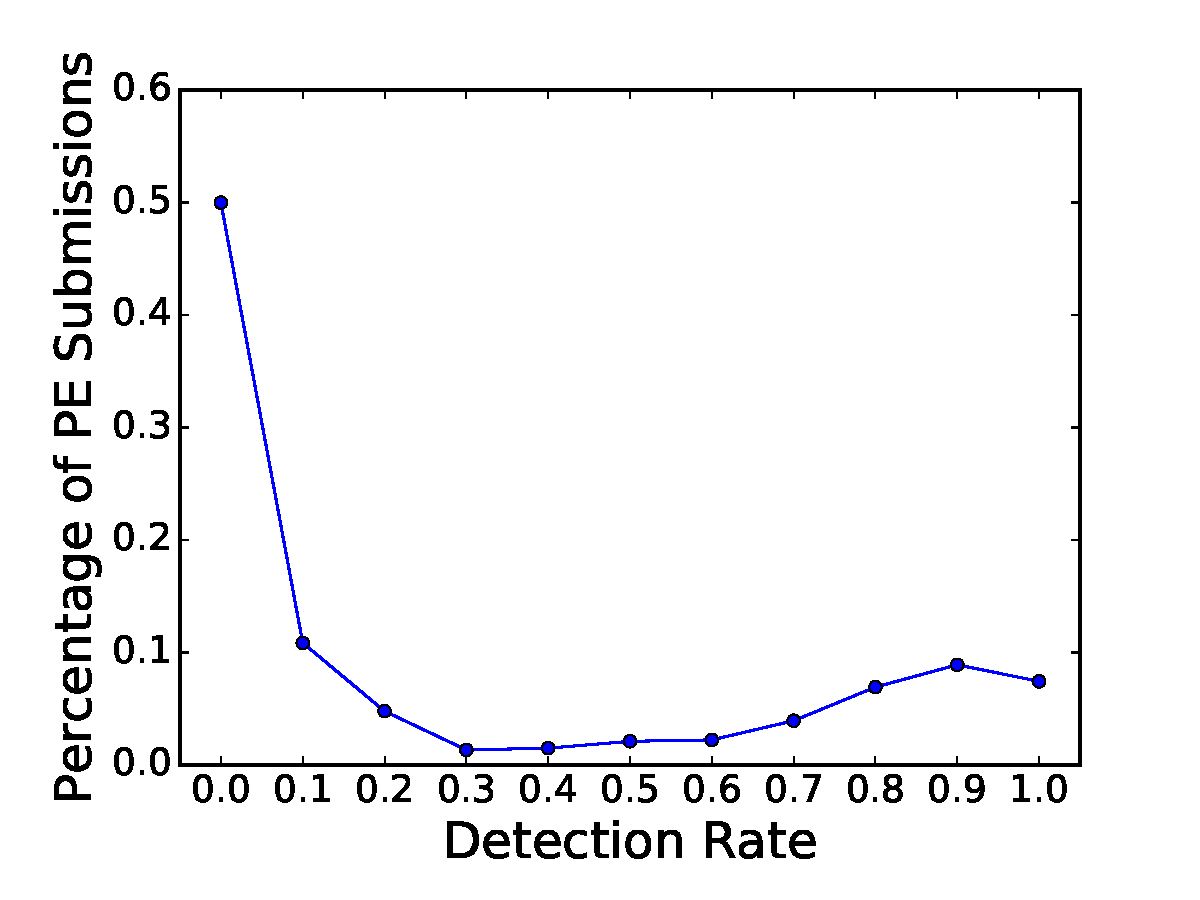
\includegraphics[width=2in]{figure/DetectionRate}
\caption{The distribution for detection rate.
(How detection rate distributes among all PE submissions. 
Each detection rate is rounded up to nearest 0.05.)
}
\label{fig:detectiorate}
\end{center}
%\vspace{-0.25in}
\end{figure}
\noindent{\textit{\underline{Anti-virus engines and detection basic analysis.}}}
After learning the basic properties of submissions and submission sources, 
we now move to the basic analysis of anti-virus engines and their detection of malware.
%As shown in Table~\ref{tab:fields}, 
%total field is to represent the number of used anti-virus engines. 
Figure~\ref{fig:vendornum} shows the distribution of the number of anti-virus engines used by \vt\ on submissions. 
More than 99\% of PE submissions are analyzed by at least 50 anti-virus engines. 
We suspect that \vt\ sets some threshold when running anti-virus engines and 
will abort an engine when it takes too long to run on a submission,
causing few submissions having fewer than 50 engines.
%Some anti-virus engines will label a submitted PE file as malware, 
%while others will not. 
%Positives field in Table~\ref{tab:fields} represents the number of anti-virus engines labeling the submission as malwares. 

For the same submission, different anti-virus engines can make different detection results, \ie, some mark the submission as malware while others don't.
To quantify the detection results of a submission,
we use a value we call {\em Detection Rate}.
Detection rate represents the percentage of engines labeling the submission as malware. 

$$ \textrm{\textit{Detection Rate}} = \dfrac{positives}{total + 1}$$

We add one to {\bf total} to avoid divide-by-zero exception, and more importantly, 
to have higher detection rate to submissions labeled as malwares by more engines.
For example, submissions analyzed by 50 engines and detected by 50 engines 
has a higher detection rate 
than submissions analyzed by one engine and detected by one engine. 
%This formula shares the same intuition from previous work~\cite{GuoICSE2010}, when computing reputations for bug reporters. 
%A larger detection rate usually indicates a more malicious malware suggested by analyzed anti-virus engines. 

Figure~\ref{fig:detectiorate} shows the distribution of detection rates over all \pe\ submissions.
We seperately consider submissions made by normal users and by anti-virus vendors 
(as defined above).
Interestingly, overall most submissions to \vt\ are likely to be benign files, \ie, has low detection rate.
Around half of the submissions were labeled as benign by all engines (a detection rate of zero),
and only 31.5\% submissions were labeled as malware by at least half of the engines.
Surprisingly, the detection rates of submissions made by normal user and by anti-virus vendors are very similar.
\yiying{any guess why?}

\if 0
Some anti-virus engines can produce different detection results when analyzing the same file under different submissions.
We assume there is influence among different anti-virus vendors, 
and this influence is a very important reason causing engines to change their results.
We will discuss how we model this influence and how to predict possible detection result change by using our model in Section~\ref{sec:influ}.
\fi

{\bf Observation 3:} 
{\em Most submissions to \vt\ are labeled as benign and 
submissions made by normal user and by anti-virus vendors have similar probabilities of being labled as malware.}

\subsection{Caveats}
Like all other empirical study works, 
our findings and conclusions need to be considered with our methodology in mind. 
We use the distribution API provided by \vt\ to download submissions' metadata 
from VirusTotal. 
There is no guarantee that this API returns all submissions to \vt.
%all data can be successfully downloaded. 
It could be possible that some files are submitted to VirusTotal, 
but are not downloaded. %we fail to get their information from VirusTotal.
Although we have collected huge amount of malware information from VirusTotal,
we do believe that there are malwares never submitted to VirusTotal, 
or submitted to VirusTotal much later than they appear in the real world. 
However, there are no conceivable ways to study them.
We believe that the 4-month malware information we collect can serve as a representative sample for malwares in the real world. 
